\section[Desenvolvimento do Projeto]{Desenvolvimento do Projeto}

Esta seção apresenta informações relativas ao desenvolvimento do projeto: localização do código-fonte e documentação, arquitetura e tecnologias utilizadas, e protótipos de tela desenvolvidos. Todas essas informações podem ser encontradas na wiki: \url{https://tools.ages.pucrs.br/totem-interativo/wiki/-/wikis/home}.

\subsection{Repositório do Código Fonte do Projeto}
  Todo o código do projeto encontra-se distribuído em dois repositórios:
\begin{itemize}
    \item código do \textit{backend}: \url{https://tools.ages.pucrs.br/totem-interativo/backend};
    \item código do \textit{frontend}: \url{https://tools.ages.pucrs.br/totem-interativo/frontend}.
\end{itemize}

Há, ainda, um terceiro repositório, usado somente para abrigar a wiki do projeto: \url{https://tools.ages.pucrs.br/totem-interativo/wiki/-/wikis/home}.

\subsection{Banco de Dados Utilizado}
  Para o desenvolvimento do projeto, optamos pelo SQLite como sistema de gerenciamento de banco de dados. Essa escolha foi estratégica, considerando dois fatores críticos: a necessidade de operação \textit{offline} e as limitações de \textit{hardware} dos totens. O SQLite, sendo extremamente leve e eficiente, consome recursos mínimos de memória e processamento, ideal para dispositivos com capacidade limitada.

  O banco foi estruturado para gerenciar informações de feiras e eventos de forma otimizada. A arquitetura priorizava consultas rápidas e diretas, organizando dados de visitantes (\textit{leads}), expositores, produtos e categorias para minimizar operações complexas.

  A tabela \textit{Lead} constituía o núcleo do sistema, armazenando dados completos dos visitantes --- informações pessoais, profissionais e suas interações com o totem. Cada \textit{lead} era vinculado às categorias de interesse e expositores pesquisados, criando um perfil detalhado de comportamento.

  Os expositores eram organizados com suporte a múltiplas categorias, incluindo o atributo ``Predio'' --- adição fundamental para o caso de uso do Tecnopuc, permitindo localização física precisa dentro do parque tecnológico. O sistema de categorização hierárquico (categorias e subcategorias) foi implementado priorizando \textit{performance}, com índices estratégicos para acelerar as buscas mais frequentes. A Figura~\ref{fig:totem-mr} apresenta o modelo relacional do banco de dados. A modelagem completa do banco de dados está disponível na wiki do projeto: \url{https://tools.ages.pucrs.br/totem-interativo/wiki/-/wikis/banco-de-dados}.

\begingroup
\setlength{\intextsep}{6pt}
\begin{figure}[H]
    \centering
    \small
    \caption{Modelo relacional do banco de dados}
    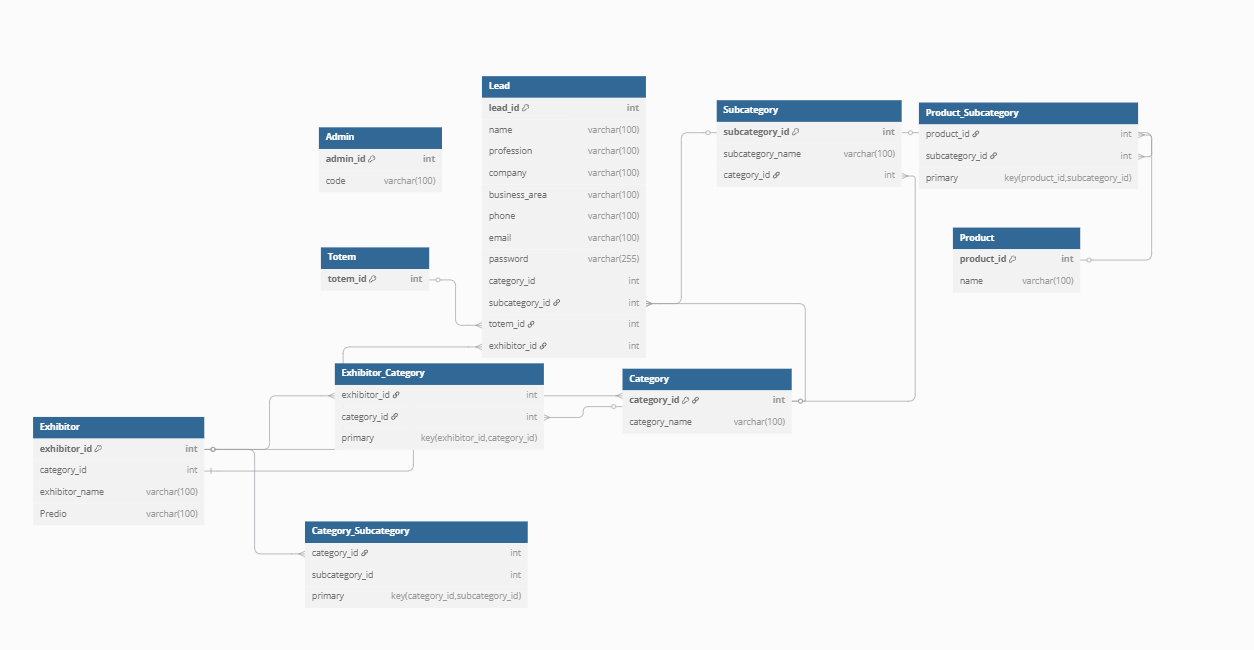
\includegraphics[width=0.72\linewidth]{conteudo/4 - ages III/images/fig7-modelo-relacional.png}

    Fonte: Documentação do projeto
    \label{fig:totem-mr}
\end{figure}
\endgroup

  A escolha do SQLite provou-se acertada para o contexto do projeto. Sua natureza \textit{serverless} elimina \textit{overhead} de comunicação, seu \textit{footprint} mínimo preserva recursos do sistema, e sua capacidade de operar em memória garante respostas rápidas. A estrutura foi projetada evitando junções múltiplas e subconsultas complexas, garantindo fluidez mesmo em \textit{hardware} básico. Essa combinação de banco leve com modelagem eficiente demonstrou que é possível criar sistemas robustos operando sob severas restrições de \textit{hardware}, proporcionando experiência responsiva aos usuários das feiras.

\subsection{Arquitetura Utilizada}
  O Totem Interativo adotou uma arquitetura cliente-servidor, com separação explícita entre o \textit{frontend} --- a aplicação que rodava no próprio totem --- e o \textit{backend}, responsável pela lógica de negócio e pelo acesso aos dados. Os dois lados comunicavam-se exclusivamente por uma \ac{api} \ac{rest} sobre \ac{http}, o que permitiu desenvolver as camadas em paralelo, isolar responsabilidades e evoluir cada parte de forma independente.

  Essa separação atendia a uma restrição central do projeto: como o totem precisava operar mesmo sem conexão externa, o \textit{frontend}, o \textit{backend} e o banco de dados eram executados localmente no próprio equipamento, e a \ac{api} atuava como a única fronteira entre a interface e os dados. A Figura~\ref{fig:totem-arquitetura} ilustra esse fluxo: a interface em Next.js consome a \ac{api} em NestJS por meio do cliente \ac{http} Axios, que por sua vez acessa o banco SQLite. O diagrama também distingue os dois perfis de uso --- o visitante, que consulta as informações no totem, e o administrador, que cadastra e gerencia os dados. As subseções seguintes detalham cada lado.

\begin{figure}[H]
    \centering
    \small
    \caption{Arquitetura do Totem Interativo e fluxo de comunicação do \textit{frontend}}
    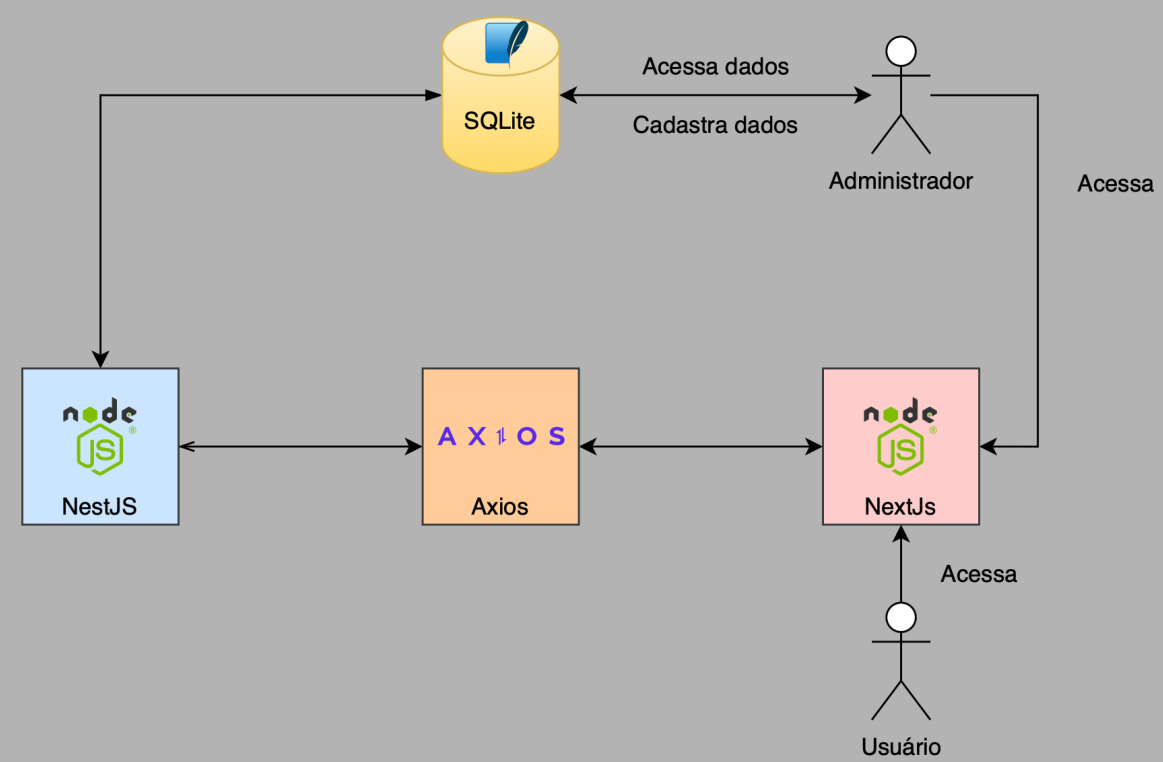
\includegraphics[width=0.85\linewidth]{conteudo/4 - ages III/images/fig-arquitetura-fluxo.png}

    Fonte: Wiki do projeto
    \label{fig:totem-arquitetura}
\end{figure}

\subsubsection{Frontend}
  A arquitetura do \textit{frontend} foi concebida para oferecer uma aplicação interativa com renderização 3D. A estrutura modular facilitou tanto o desenvolvimento quanto a manutenção.

  Os componentes da interface foram organizados em grupos lógicos:
\begin{itemize}
    \item \textit{dropdown}: para menus de seleção e filtros;
    \item \textit{map}: responsável pela renderização e interação com o mapa 3D;
    \item \textit{searchbar}: para funcionalidades de busca;
    \item \textit{sidebar}: para navegação e exibição de informações contextuais.
\end{itemize}

  A comunicação com o \textit{backend} foi centralizada na camada de \textit{services}, atuando como um ponto único de integração com as \acp{api}. O gerenciamento de estados globais foi feito via \textit{contexts}, e lógicas reutilizáveis, como o \textit{logout} automático por inatividade, foram isoladas em \textit{hooks}.

  Recursos estáticos essenciais para o mapa 3D foram estrategicamente organizados:
\begin{itemize}
    \item \textit{models}: arquivos de geometria dos edifícios;
    \item \textit{textures}: materiais visuais aplicados aos modelos;
    \item \textit{fonts}: tipografias personalizadas para a identidade visual;
    \item \textit{assets}: recursos gráficos gerais da aplicação.
\end{itemize}

  As rotas da aplicação eram diferenciadas conforme o perfil do usuário: visitantes acessavam a interface principal do totem, enquanto administradores contavam com páginas específicas para importação de dados (\textit{admin-import}) e exportação de relatórios (\textit{admin}). A funcionalidade de \textit{QR Code} possuía um módulo próprio com componentes dedicados.

\subsubsection{Backend}
  A arquitetura do \textit{backend} adotou padrões de desenvolvimento em camadas, garantindo uma clara segregação de responsabilidades e facilitando os processos de teste e manutenção.

  A estrutura de camadas implementada era composta por:
\begin{itemize}
    \item \textit{Controllers}: atuavam como ponto de entrada para as requisições \ac{http};
    \item \textit{Services}: encapsulavam toda a lógica de negócio da aplicação;
    \item \textit{\acp{dto}}: definiam os contratos de dados para entrada e saída;
    \item \textit{Entities}: representavam as estruturas do banco de dados;
    \item \textit{Modules}: agrupavam logicamente as funcionalidades.
\end{itemize}

  Aspectos transversais foram concentrados no diretório \textit{common}:
\begin{itemize}
    \item \textit{Guards}: para proteção de rotas administrativas;
    \item \textit{Filters}: para tratamento padronizado de erros;
    \item \textit{Mapper}: para transformações entre diferentes representações de dados.
\end{itemize}

  O armazenamento local foi estruturado no diretório \textit{database}, contendo o arquivo principal SQLite.

  O fluxo de dados seguia um padrão consistente: as requisições chegavam aos \textit{controllers}, eram validadas pelos \textit{DTOs}, processadas pelos \textit{services} (que interagiam com as \textit{entities}), e então retornavam respostas estruturadas. As operações administrativas incluíam \textit{endpoints} especializados para importação em massa via \ac{csv} e exportação de dados agregados.

  A estrutura de testes replicava a organização principal, com diretórios específicos para \textit{controllers} e \textit{services}, assegurando uma cobertura adequada das funcionalidades críticas.

\subsection{Protótipos das Telas Desenvolvidas}
  Os protótipos deste projeto estão disponíveis na wiki do projeto: \url{https://tools.ages.pucrs.br/totem-interativo/wiki/-/wikis/mockups}.

  O \textit{design} da aplicação, como pode ser visto a seguir, poderia ser aprimorado, porém à época era considerado agradável, algo que o cliente aprovou bastante. As telas apresentadas a seguir contemplam o fluxo do visitante --- composto pela tela inicial, pelos menus e pela busca de expositores --- e o fluxo do administrador, responsável pela importação dos dados e pela configuração do evento.

  A Figura \ref{fig:totem-tela-inicial} apresenta a tela inicial do totem, com o mapa interativo utilizado para orientar o visitante pelo espaço do evento.

\begingroup
\setlength{\intextsep}{6pt}
\begin{figure}[H]
    \centering
    \small
    \caption{Tela inicial com mapa interativo}
    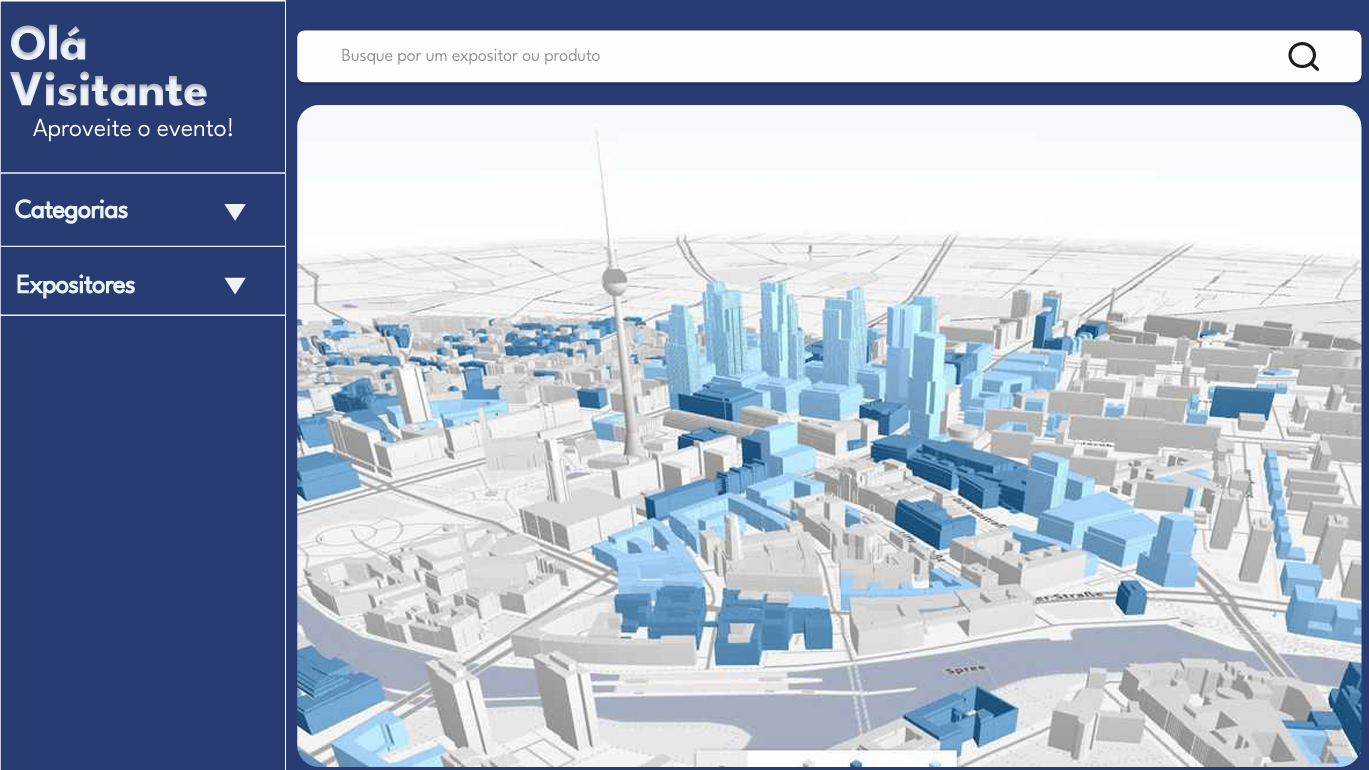
\includegraphics[width=0.9\linewidth,height=0.28\textheight,keepaspectratio]{conteudo/4 - ages III/images/tela-inicial-mapa.png}

    Fonte: Wiki do projeto
    \label{fig:totem-tela-inicial}
\end{figure}
\endgroup

  A Figura \ref{fig:totem-menus} exibe os menus de categorias e de expositores, que organizam a navegação pelo conteúdo disponível.

\begin{figure}[H]
    \centering
    \small
    \caption{Menus de categorias e expositores}
    \begin{minipage}{0.38\linewidth}
        \centering
        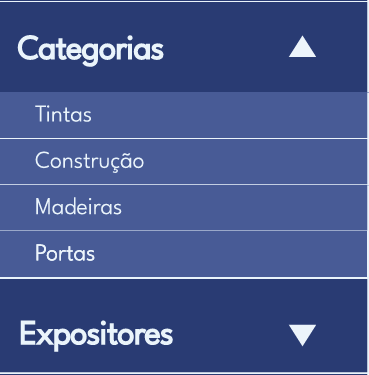
\includegraphics[width=\linewidth,height=0.3\textheight,keepaspectratio]{conteudo/4 - ages III/images/menu-categorias.png}
    \end{minipage}\hfill
    \begin{minipage}{0.38\linewidth}
        \centering
        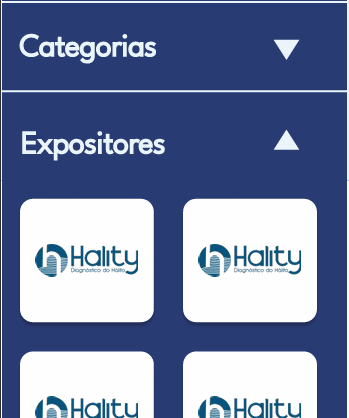
\includegraphics[width=\linewidth,height=0.3\textheight,keepaspectratio]{conteudo/4 - ages III/images/menu-expositores.png}
    \end{minipage}

    Fonte: Wiki do projeto
    \label{fig:totem-menus}
\end{figure}

  A Figura \ref{fig:totem-busca} mostra a busca de expositores no totem, que permite localizar rapidamente um expositor específico.

\begin{figure}[H]
    \centering
    \small
    \caption{Busca de expositores}
    
\includegraphics[width=0.9\linewidth,height=0.34\textheight,keepaspectratio]{conteudo/4 - ages III/images/busca-expositores.png}

    Fonte: Wiki do projeto
    \label{fig:totem-busca}
\end{figure}

  Por fim, a Figura \ref{fig:totem-config-admin} abrange o fluxo do administrador, responsável pela importação dos dados e pela configuração do evento.

\begin{figure}[H]
    \centering
    \small
    \caption{Tela de configurações do administrador}
    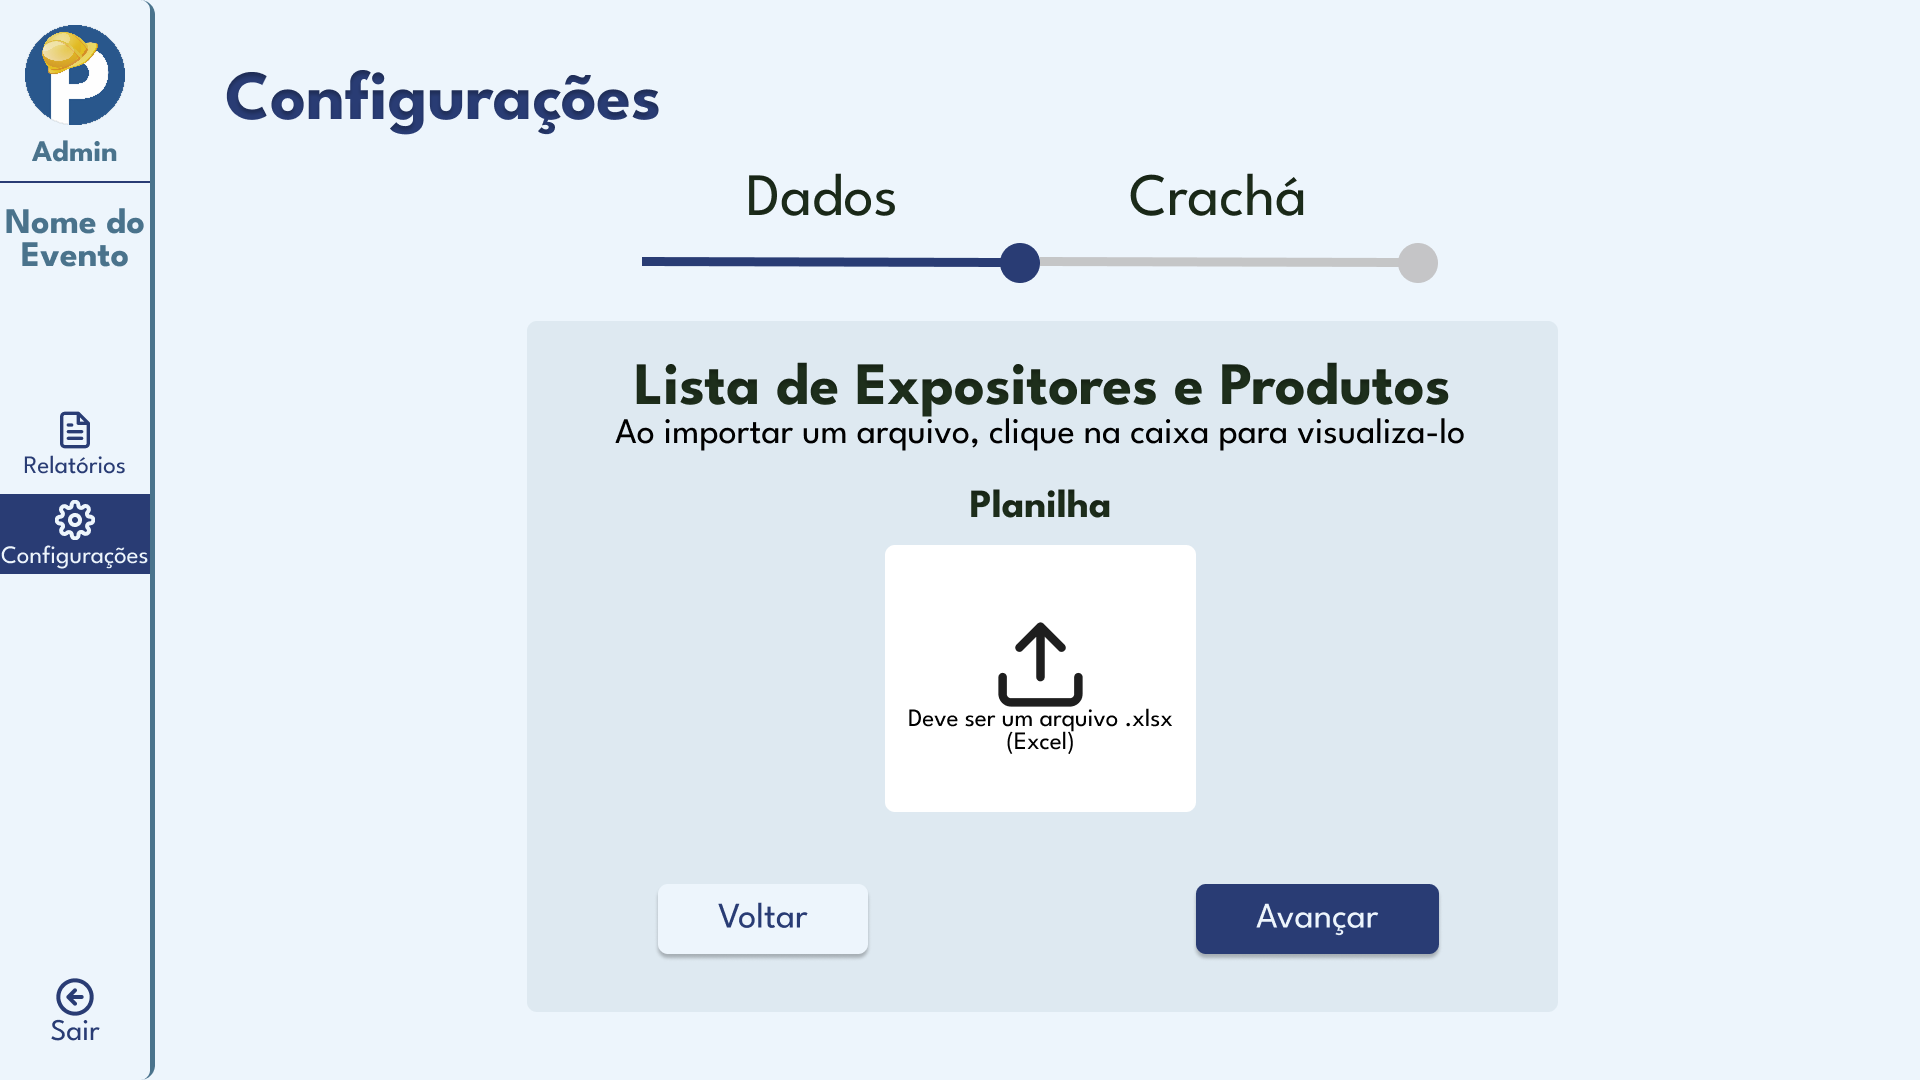
\includegraphics[width=0.85\linewidth,height=0.34\textheight,keepaspectratio]{conteudo/4 - ages III/images/config-admin.png}

    Fonte: Wiki do projeto
    \label{fig:totem-config-admin}
\end{figure}

\subsection{Tecnologias Utilizadas}
  Nesta seção são apresentadas as principais tecnologias empregadas no desenvolvimento do projeto Totem Interativo, destacando suas contribuições para o sucesso da implementação.

\begin{itemize}
    \item \textbf{React} \parencite{react}: Biblioteca JavaScript de código aberto para construção de interfaces de usuário reativas e componentes reutilizáveis, fundamental para criar a interface interativa do totem com atualizações dinâmicas.
    \item \textbf{Three.js} \parencite{threejs}: Biblioteca JavaScript para renderização 3D no navegador, responsável pela criação e manipulação do mapa tridimensional interativo, permitindo visualização imersiva dos espaços e interações com elementos 3D.
    \item \textbf{Next.js} \parencite{nextjs}: \textit{Framework} React para desenvolvimento \textit{web} com renderização híbrida e otimizações automáticas de \textit{performance}, garantindo resposta rápida mesmo em \textit{hardware} limitado.
    \item \textbf{Node.js} \parencite{nodejs}: Ambiente de execução JavaScript \textit{server-side} com natureza assíncrona e eficiência no gerenciamento de I/O, ideal para múltiplas requisições simultâneas.
    \item \textbf{NestJS} \parencite{nestjs}: \textit{Framework} progressivo para Node.js que permite construção de aplicativos escaláveis com arquitetura modular e suporte nativo para TypeScript.
    \item \textbf{TypeScript} \parencite{typescript}: \textit{Superset} do JavaScript que adiciona tipagem estática opcional, reduzindo \textit{bugs} em tempo de desenvolvimento e facilitando manutenção do código.
    \item \textbf{Swagger} \parencite{swagger}: Ferramenta para documentação e testes interativos de \acp{api} RESTful, integrada ao NestJS para gerar documentação automática dos \textit{endpoints}.
    \item \textbf{SQLite} \parencite{sqlite}: Sistema de banco de dados relacional \textit{serverless} e baseado em arquivo único, escolhido por sua leveza e capacidade de operar sem dependências externas em ambiente \textit{offline}.
\end{itemize}
